\section{Results}\label{Results}
	
	The performance of processed camera data can be evaluated with metrics presented in \cite{Reway} which are realized like introduced in \cref{sssec:eval}. The metrics are validated by comparing two identical Rosbag files. This ensures that the implementation of the evaluation functions are correctly.
	Considering the objects lists created by data processing it is noticeable that the camera data is quite different from the \ac{GT} data. Because the simulation is subject to near real-time requirements, a fast processing time is essential. The evaluation and tracking of camera data needs at least 1 second, hence is not fast enough to deliver comparable results. This delay leads to a perceptible offset in the visualization, therefore it is hardly possible to measure the precision of \ac{YOLO} and the calculation.
	\Cref{fig:result} shows the distance of an object in x direction from \ac{GT} data and camera data. Moreover, this figure  makes the time difference between \ac{GT} and camera data very clearly. The \ac{GT} stream ends sending after about nine seconds, because the used sensor suite cannot recognize an object anymore. Certainly, the camera data  sends the comparable object list after another two seconds, so that a correct evaluation can not be carried out. Furthermore, minor errors occur with slightly misplaced bounding boxes by \ac{YOLO} and detecting the object precisely within the given bounding box. This influences following values like calculation of the object length and object height.\\
	
	\begin{figure}[b]
		\centering
		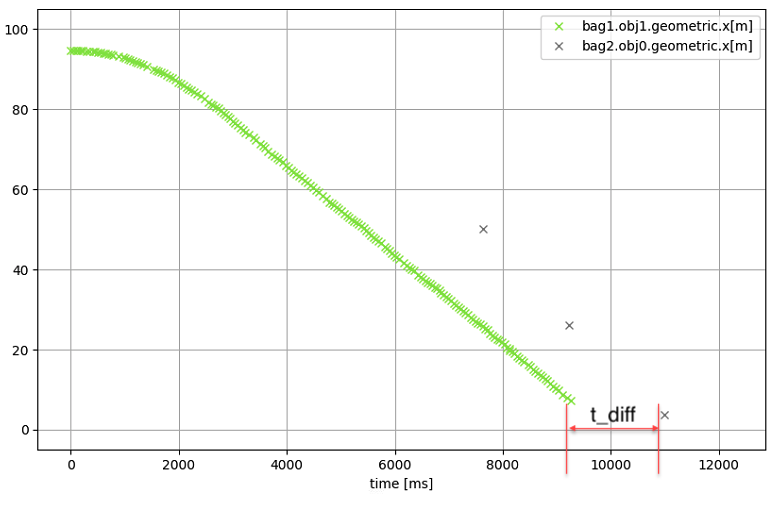
\includegraphics[width=0.5\textwidth]{result_graphic.png}
		\caption{Post-processing GT (green)/ Camera Data (gray)}
		\label{fig:result}
	\end{figure}
%	For the given scenario the reached performance is shown in table \ref{tab:res}.
%	
%	\begin{table}[h]
%		\caption{Performance results}
%		\begin{tabularx}{\columnwidth}{XXXX}
%			\toprule
%			\textbf{threshold} & $t=0.5$ & $t=0.6$ & $t=0.7$ \\
%			\toprule
%			Precision & ... & ... & ... \\
%			\midrule
%			Recall & ... & ... & ... \\
%			\midrule		
%			FPPI & ... & ... & ... \\
%			\midrule
%			MOTA & ... & ... & ... \\
%			\midrule
%			MOTP & ... & ... & ... \\
%			\bottomrule
%		\end{tabularx}
%		\label{tab:res}
%	\end{table}